\documentclass[11pt, a4paper]{book}
\usepackage[french]{babel}
\usepackage[utf8]{inputenc}
\usepackage{answers}

\usepackage{hyperref}
\usepackage{multicol}

\usepackage[table,xcdraw]{xcolor}
\usepackage{listings}
\definecolor{ForestGreen}{RGB}{34,139,34}


\usepackage{enumitem}

\AtBeginDocument{\def\labelitemi{$\bullet$}}


\newcommand{\py}{\lstinline{Python} }


\definecolor{backcolour}{rgb}{0.95,0.95,0.92}

\lstset{%
	language         = Python,
	backgroundcolor  = \color{backcolour},
	basicstyle       = \ttfamily, % \upshape\ttfamily,
	keywordstyle     = \bfseries\color{blue}, %\bfseries,
	stringstyle      = \color{magenta},
	commentstyle     = \color{ForestGreen},
	alsoletter = > ,
	morekeywords = {>>>,as,assert,False,None, nonlocal,True, with,yield , <<, >>, :},
	showstringspaces = false,
	numbers=left,
	stepnumber=1,
	literate={à}{{\`{a}}}1 {é}{{\'e}}1 {è}{{\`{e}}}1 {ê}{{\^{e}}}1 {Ê}{{\^{E}}}1 {î}{{\^i}}1 {ô}{{\^{o}}}1 {ç}{{\c{c}}}1 {Ç}{{\c{C}}}1
}

\newcommand{\itemb}[1]{\item \textbf{#1}}

\usepackage{fancyhdr}  %package pour en-tetes et pied de pages
\usepackage{sectsty} % Permet de faire des modifications de police dans diverses sections des "headings" (cf. modif presentation de la page)
\pagestyle{fancy}       %Style pour en-tetes et pieds de pages
\fancyhead[CO,CE]{\sc Série 1\hspace{0.5mm}}
\fancyhead[RO,LE]{Collège Sismondi}  % LaTeX/TEX define \strut to be an invisible box of width zero that extends just enough above and below the baseline. Cela permet d'augementer légèrement la taille en bas de la box de manière à ce qu'elle soit collée à la ligne.
\fancyhead[LO,RE]{\small\ \textsl{1\textsuperscript{ère} année - DO Informatique}}
\fancyfoot[RO,LE]{2021 - 2022}
\fancyfoot[LO,RE]{\small }
\fancyfoot[CO,CE]{\thepage}

\fancyhfoffset[l]{1.2cm} % le "l" en paramètre permet d'indiquer qu'on ne veut modifier que la marge à gauche.
\renewcommand{\headrule}{{%
		\hrule \headwidth \headrulewidth \vskip-\headrulewidth}}
\renewcommand\footrulewidth{\headrulewidth}
\renewcommand{\footrule}{{%
		\vskip-\footruleskip\vskip-\footrulewidth
		\hrule \headwidth \footrulewidth\vskip\footruleskip}}

\usepackage{tikz}
%-------------------------------------------------------------------------------
%---- Eclairage : en encadré sur fond jaune avec symbôle "ampoule" à gauche ----
%-------------------------------------------------------------------------------
\definecolor{coleclairage}{RGB}{255 , 221 , 156}
\definecolor{contoureclairage}{RGB}{255 , 192 , 0}
\newenvironment{eclairage}
{
	\begin{center}%
		\begin{tikzpicture}%
			\node[rectangle, draw=contoureclairage, top color=coleclairage!50, bottom color=coleclairage!140, rounded corners=5pt, inner xsep=5pt, inner ysep=6pt, outer ysep=10pt]\bgroup                     
			\begin{minipage}{0.98\linewidth}
				\begin{minipage}{0.08\linewidth}\centerline{
\includegraphics[scale=1]{Symbole_eclairage.png}}\end{minipage}
				\begin{minipage}{0.89\linewidth}\itshape\footnotesize
				}
				{                		
				\end{minipage}
			\end{minipage}\egroup;%
		\end{tikzpicture}%
	\end{center}%
}

%-------------------------------------------------------------------------------
%---- apprendre : en encadré sur fond jaune avec symbôle "ampoule" à gauche ----
%-------------------------------------------------------------------------------
\definecolor{colapprendre}{RGB}{50,205,50}
\definecolor{contourapprendre}{RGB}{34,139,34}
\newenvironment{apprendre}
{
	\begin{center}%
		\begin{tikzpicture}%
			\node[rectangle, draw=contourapprendre, top color=colapprendre!10, bottom color=colapprendre!50, rounded corners=5pt, inner xsep=5pt, inner ysep=6pt, outer ysep=10pt]\bgroup                     
			\begin{minipage}{0.98\linewidth}
				\begin{minipage}{0.08\linewidth}\centerline{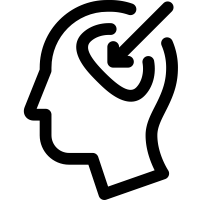
\includegraphics[width=30px]{Symbole_learn.png}}\end{minipage}
				\begin{minipage}{0.89\linewidth}\itshape\footnotesize
				}
				{                		
				\end{minipage}
			\end{minipage}\egroup;%
		\end{tikzpicture}%
	\end{center}%
}

\definecolor{colimportant}{RGB}{247 , 189 , 164}
\definecolor{contourimportant}{RGB}{237 , 125 , 49}
\newenvironment{important}
{
	\begin{center}%
		\begin{tikzpicture}%
			\node[rectangle, draw=contourimportant, top color=colimportant!50, bottom color=colimportant!140, rounded corners=5pt, inner xsep=5pt, inner ysep=6pt, outer ysep=10pt]\bgroup                     
			\begin{minipage}{0.08\linewidth}\centerline{
\includegraphics[scale=0.8]{Symbole_attention.png}}\end{minipage}
			\begin{minipage}{0.89\linewidth}
			}
			{                		
			\end{minipage}\egroup;
		\end{tikzpicture}%
	\end{center}%
}

%-----------------------------------------------------------------
%---- Modification présentation de la page: marges de la page ----
%-----------------------------------------------------------------
%\addtolength{\hoffset}{-1in}              % 1
%\addtolength{\voffset}{-1in}              % 2
\addtolength{\oddsidemargin}{-0.1 in} % 3
\addtolength{\evensidemargin}{-1in} % 3
\addtolength{\topmargin}{-1in}       % 4
\addtolength{\headheight}{6pt}       % 5
%\addtolength{\headsep}{-0.2cm}           % 6
\setlength{\textheight}{26cm}    % 7
\setlength{\textwidth}{16.5cm}      % 8
\addtolength{\marginparsep}{0pt}      % 9
\setlength{\marginparwidth}{0pt}   % 10
\addtolength{\footskip}{-1mm}           %11

\setlength{\parindent}{0em}% pas d'indentation


% Customiser le nom des sections
\usepackage{titlesec}
\titleformat{\section}[hang]{\Large \bfseries}{Série \thesection:\ }{0pt}{}

\renewcommand{\familydefault}{\sfdefault} % pour avoir des polices san serif

\newtheorem{Exc}{Exercice}
\Newassociation{correction}{Soln}{mycor}
\renewcommand{\Solnlabel}[1]{\bfseries Ex #1 }
\def\exo#1{%
	\futurelet\testchar\MaybeOptArgmyexoo}
\def\MaybeOptArgmyexoo{
	\ifx[\testchar \let\next\OptArgmyexoo
	\else \let\next\NoOptArgmyexoo \fi \next}
\def\OptArgmyexoo[#1]{%
	\begin{Exc}[#1]\normalfont}
	\def\NoOptArgmyexoo{%
		\begin{Exc}\normalfont}
		\newcommand{\finexo}{\end{Exc} \vspace{3mm}}
	\newcommand{\flag}[1]{}
	\newcommand{\entete}[1]

\newcommand{\getexocompteur}{{\the\numexpr \arabic{Exc}  \relax}}	
	
\newcommand{\eexo}{\vspace{5mm}} % espace pour séparer les exercices
\usepackage{minted}
\pgfplotsset{compat=1.17}
\begin{document}

\setcounter{chapter}{3}

\chapter{Notion de fichiers}

\section{Fichiers}
\subsection{Introduction}

Un fichier informatique est un ensemble de données numériques que l'on souhaite faire persister en le stockant sur un support permanent. Un fichier peut être :une image, un film, du texte, un programme source, un programme exécutable, un fichier compressé, etc. Quant au support permanent (cf. chapitre Ordinateur) il s'agit d'un disque dur, un DVD, une clé USB, etc.

Un disque stocke simplement une suite de bits, une suite de 0 et de 1. Le nombre de bits qu’un disque peut stocker est appelé sa capacité : par exemple un disque d’un téraoctet (binaire) peut stocker 240 mots de 8 bits, soit un peu plus de huit mille milliards de bits. On peut donc facilement stocker un texte, une image, un son ou un programme sur un tel disque. Cependant, comme on souhaite souvent stocker sur un disque plusieurs images, textes, etc., il faut diviser les huit mille milliards de bits dont le disque est constitué en plusieurs espaces plus petits, que l’on appelle des fichiers. Un fichier est simplement une suite de 0 et de 1, à laquelle on associe un nom. Par exemple, le texte "Je pense, donc je suis.» se représente en ASCII étendu comme la suite de 184 bits suivante :

\begin{minted}{latex}
0100101001100101001000000111000001100101011011
1001110011011001010010110000100000011001000110
1111011011100110001100100000011010100110010100
1000000111001101110101011010010111001100101110
\end{minted}

Il est possible de stocker cette suite de bits sur un disque en lui donnant le nom cogito.txt, l’extension txt indiquant que cette suite de bits exprime un texte en ASCII. L’extension détermine le type d’information exprimé (texte, image, son, etc.) et le format utilisé pour l’exprimer.

\subsection{Nom de fichier}
Un fichier comporte donc un {\it nom\_de\_fichier}  qui permet de l’identifier et d’y accéder. Ce nom est généralement constitué de deux parties séparées par un point. Par exemple, le fichier nommé {\it Recette\_tarte\_aux\_pommes.odt} se décompose :

\begin{center}
\begin{tikzpicture}
	\filldraw[fill=lightgray] (0,0.8) rectangle (10,1.6);
	\draw (0,0) rectangle (10,0.8)
			(0,0) rectangle (10,1.6)
			(0,0) rectangle (5,1.6)
			(0,0) rectangle (7.5,1.6);
	\draw (2.5,1.2) node {\bf Nom du fichier};
	\draw (6.25, 1.2) node {\bf .};
	\draw (8.75,1.2) node {\bf Extension};
	
	\draw (2.5,0.4) node {\it Recette\_tarte\_aux\_pommes};
	\draw (6.25, 0.4) node {\bf .};
	\draw (8.75,0.4) node {\it odt};
			
\end{tikzpicture}
\end{center}

Comme le nom du fichier identifie son contenu, il est important de choisir un nom explicite. En effet, si vous nommez votre rédaction de français avec le nom suivant :

$\rightarrow$ {\it Rédaction\_le\_petit\_prince.odt} : Ce fichier désignera probablement une rédaction avec comme sujet le petit prince.

Par contre, si vous choisissez le nom :

$\rightarrow$ {\it mon\_fichier.odt} : Ce nom ne donne aucune information sur son contenu. On n’aura strictement aucune idée de quoi il s’agit sauf qu’il s’agit d’un fichier !
\begin{remarques}
\begin{enumerate}
\item[]
\item Pour l’utilisateur·trice, il est donc utile et important de bien choisir un nom qui identifie le contenu de son fichier.
\item Vous remarquez également que des caractères soulignés ( \_ ) ont été utilisés dans la nomenclature. En effet, pendant longtemps, les espaces n’étaient pas autorisés pour nommer des fichiers, car les espaces étaient utilisés comme séparateurs de nom de fichier ! Actuellement, l’espace est accepté sur la plupart des systèmes, mais il existe toujours de vieux programmes qui refusent un espace dans le nom du fichier ou génère une erreur.
\item Les caractères accentués (é ê è ü à ä î ô û) étaient également interdits. C’est pour cette raison que l’on trouve souvent des fichiers qui n’ont pas d’accent (merci l’orthographe me direz-vous). À noter qu’il subsiste également d’autres caractères qui sont interdits ou déconseillés:
\begin{itemize}
\item Microsoft Windows (interdits) $< \; >  \,  :  \;   " \;   \backslash \;  / \; \vert \; . \; ? \; *$ 
\item Gnu/Linux et Mac OS (déconseillés): $/$ * 
\end{itemize}
\item Les noms ont aussi une limite en longueur, jusqu’à 256 caractères (voir plus pour les tout nouveaux systèmes), mais dans les années 80, le système d’exploitation MS-Dos n’autorisait que 8 caractères plus le point et l’extension de 3 caractères !
\item Certains systèmes de fichier sont sensibles à la casse, mais pas Microsoft Windows. Exemple avec ces trois noms :
\begin{enumerate}[a)]
\item {\it recette\_tarte\_aux\_pommes.odt}
\item {\it Recette\_tarte\_aux\_pommes.odt}
\item {\it RECETTE\_TARTE\_AUX\_POMMES.odt}
\end{enumerate}
Ces trois fichiers indiqueront le même document pour Microsoft Windows, mais bien trois fichiers distincts pour GNU/Linux ou macOS.
\end{enumerate}
\end{remarques}

\section{Extension}
\subsection{Type d'extension}
Comme cité précédemment, l’extension est formée en général de 3 lettres, mais elle peut en contenir plus (ex. : .html), voir moins ou carrément aucune. L’extension, par convention, indique la nature du fichier. Voici quelques exemples :

\begin{center}
\begin{tikzpicture}
	\filldraw[fill=lightgray] (0,8.8) rectangle (12,8);
	\draw (12,-.8) rectangle
	(0,0) rectangle (12,0.8) rectangle (0,1.6) 
		rectangle (12,2.4) rectangle (0,3.2) 
		rectangle (12,4) rectangle (0,4.8)
		rectangle (12,5.6) rectangle (0,6.4)
		rectangle (12,7.2) rectangle (0,8);
	\draw (8,-0.8) -- (8,8.8);
	
	\draw (4,8.4) node {\bf Nature du contenu};
	\draw (10,8.4) node {\bf Extensions};
	
	\draw (4,7.6) node {Document texte libre office writer};
	\draw (10,7.6) node { odt};
	
	\draw (4,6.8) node {Document tableur libre office calc};
	\draw (10,6.8) node {ods};
	
	\draw (4,6) node {Document texte Microsoft Word};
	\draw (10,6) node {docx};
	
	\draw (4,5.2) node {Document tableur Microsoft Excel};
	\draw (10,5.2) node {xlsx};
	
	\draw (4,4.4) node {Document texte};
	\draw (10,4.4) node {txt};
	
	\draw (4,3.6) node {Exemples de formats de fichiers compressés};
	\draw (10,3.6) node {zip, 7z, rar, lzw};
	
	\draw (4,2.8) node {Exemples de formats de fichiers audio};
	\draw (10,2.8) node {mp3, wav, ogg, flac};
	
	\draw (4,2) node {Images, photos};
	\draw (10,2) node {png, jpeg, gif};
	
	\draw (4,1.2) node {Video, film};
	\draw (10,1.2) node {avi, mpg, mov, flv};
	
	\draw (4,0.4) node {Page web};
	\draw (10,0.4) node {htm, html};
	
	\draw (4,-0.4) node {Exemples de formats de fichiers de code source};
	\draw (10,-0.4) node {java, c, py};

\end{tikzpicture}
\end{center}
\subsection{Type MIME}
Les systèmes d'exploitation gnu/Linux et MacOS ne demandent pas d'extension aux différents type de fichiers. En effet, ces deux systèmes se basent sur des informations rattachées aux fichiers, les types MIME. Les types MIME sont désormais appelés "types de média Internet". Les types MIME ont été créés à l’origine pour le courrier électronique. "MIME" (Multipurpose Internet Mail Extensions) est un standard qui a été proposé par les laboratoires Bell Communications en 1991 afin d'étendre les possibilités du courrier électronique (courriel), c'est-à-dire de permettre d'insérer des documents (images, sons, texte, ...) lors d'un envoi de message électronique, mais ils se sont étendus à d’autres utilisations.

MS Windows ignore les types MIME et se base uniquement sur les extensions de fichier. Par exemple, vous pouvez avoir un fichier texte nommé "Exemple.txt". MS Windows comprend qu’il s’agit d’un fichier texte en raison de l’extension de fichier .txt. Supprimez le .txt. extension de fichier et renommer le fichier en "Exemple" sans extension de fichier. MS Windows ne saura pas quoi faire avec le fichier résultant. C’est pourquoi MS Windows vous avertit lors de la suppression de l’extension de fichier, en disant "Si vous modifiez une extension de nom de fichier, le fichier peut devenir inutilisable. Êtes-vous sûr de vouloir le changer ?". 
\begin{figure}[h!]
\centering
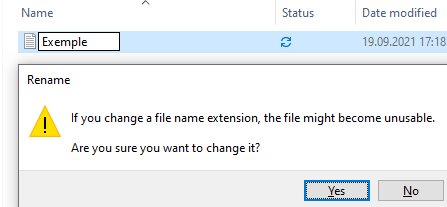
\includegraphics[width=10cm]{images/change_extension.png}
\end{figure}

Ce fichier ne deviendra pas inutilisable (pour toujours). Vous pouvez le rendre à nouveau "utilisable" en ajoutant l’extension du fichier d’origine.
C’est une des raisons principales de MS Windows de masquer les extensions de fichiers par défaut dans son explorateur de fichier. Cette option évite que les utilisateurs suppriment accidentellement l'extension d'un fichier. Des attaquants (pirates) peuvent abuser de ce comportement pour cacher du code malveillant et des virus dans des fichiers en choisissant de fausses extensions de fichiers.

Les informations sur la nature du fichier, le type MIME, sont intégrées au début du fichier lui-même. Ainsi, lorsque vous ouvrez un fichier sans extension de fichier, gnu/Linux et MacOS examineront le type MIME du fichier pour déterminer de quel type de fichier il s’agit.


\section{Organisation des fichiers}

Lorsque vous prenez une photo avec votre smartphone où se trouve-t-elle ? Quel nom de fichier identifie la photo ? Comment vous y prenez-vous pour classer vos photos ? Ne vous est-il pas arrivé de défiler les photos sur votre écran à la recherche d’une en particulier ? Comment faudrait-il procéder pour retrouver plus rapidement une photo ? Si vos photos sont classées par date et par album n’est-il pas plus simple de retrouver une photo ? Le problème dans notre cas de figure c'est que toutes les photographies se retrouvent au même endroit, sans classement, dans la mémoire permanente du téléphone mobile.

En informatique, pour organiser des fichiers, il est nécessaire de créer des dossiers (ou des répertoires). Dans un dossier, nous pouvons trouver d’autres dossiers et fichiers. Cette structure forme une hiérarchie cohérente. Organiser ses fichiers c’est comme ranger ses feuilles de cours dans plusieurs classeurs avec des pochettes et des séparateurs. Prenons l’exemple suivant pour illustrer le classement de ses feuilles de cours papier. Il s’agit donc de classer différents documents de cours dans leur classeur respectif. Dans notre illustration, nous avons choisi de créer un classeur par discipline ce qui permet, par exemple, de ranger la feuille de géographie Suisse dans la pochette Europe qui se trouve dans le classeur Géographie. Ce classeur sera rangé dans l’armoire des classeurs.

\begin{figure}[h!]
\centering
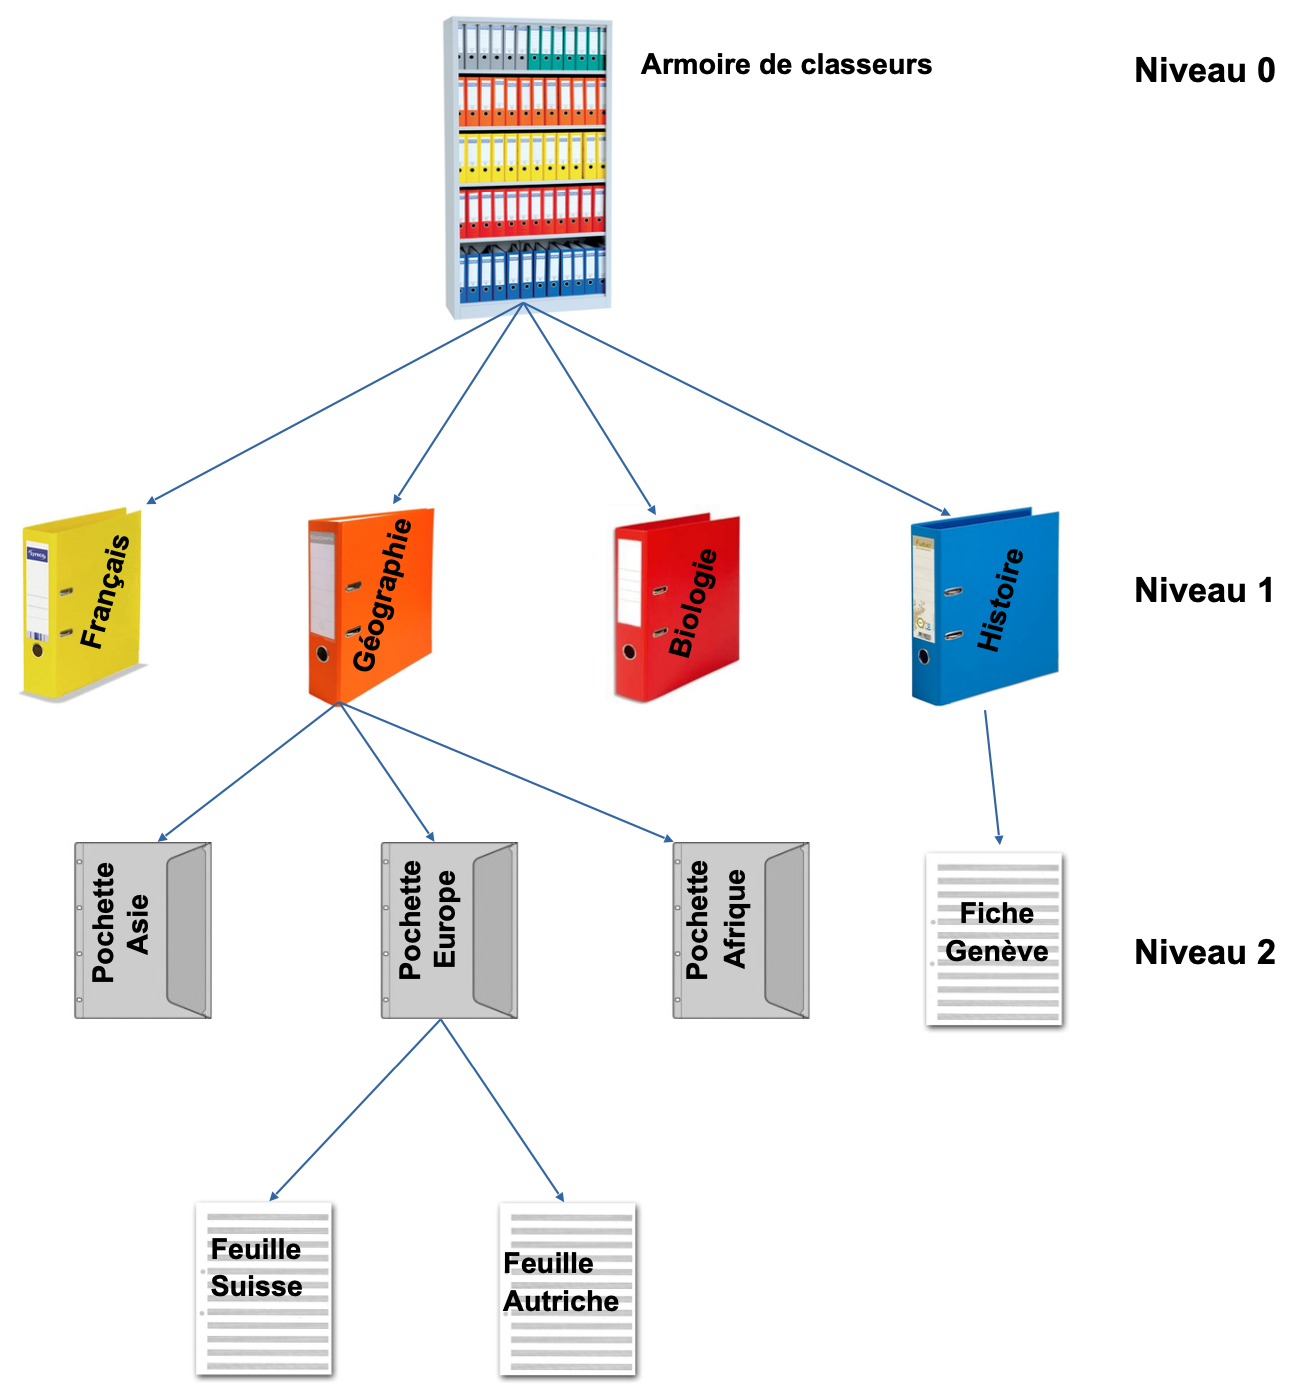
\includegraphics[width=12cm]{images/organisationfichiers}
\end{figure}

Cette structure se retrouve dans les systèmes de fichiers de manière analogue. Sous GNU/Linux ou macOS le niveau 0 se nomme la racine et le dernier niveau les feuilles (par analogie avec un arbre inversé). Le passage d’un niveau à l’autre, les branches, est décrit par un / (slash). Le chemin pour parvenir au fichier depuis la racine (niveau 0) se nomme le chemin d’accès. Il décrit précisément l’emplacement du fichier (l’itinéraire complet). On appelle une telle organisation des fichiers une organisation arborescente, car on peut la visualiser sous la forme d’un arbre.

Pour résumer: 
\begin{enumerate}[a)]
\item Un {\bf dossier} peut comporter d’autres dossiers et des fichiers.
\item Un {\bf fichier} est un ensemble organisé d'informations, désigné par un nom précis, que le système d'exploitation d'un ordinateur manipule comme une simple entité, dans sa mémoire ou sur un support de stockage.
\end{enumerate}

\begin{figure}[h!]
\centering
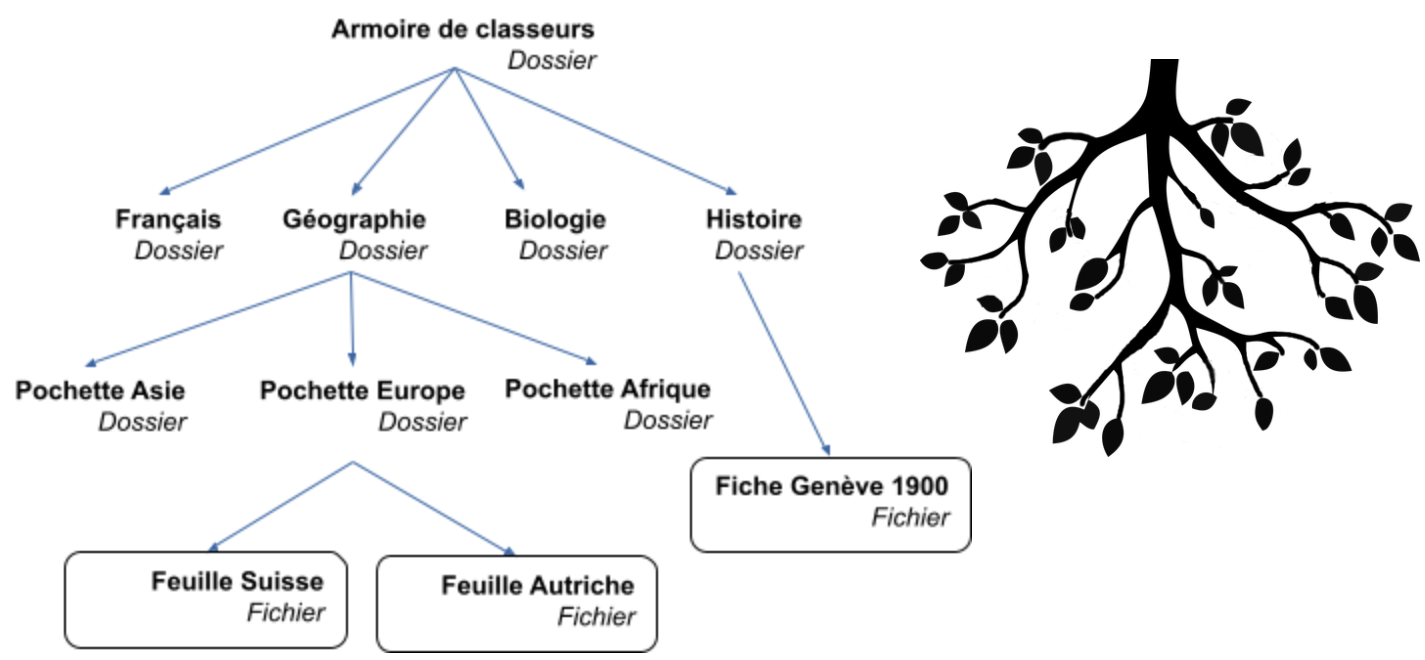
\includegraphics[width=15cm]{images/arborescence2}
\end{figure}
L’organisation arborescente des fichiers n’est pas le seul moyen de structurer l’information : elle est en concurrence avec d’autres méthodes, parmi lesquelles l’utilisation de liens hypertextes, notion qui n’a pas été inventée pour structurer l’information, mais pour simplifier le mécanisme de référence dans une page web.

% SECTION
\section{Explorateur de fichiers sous différents système d'exploitation}
Pour nous aider à parcourir l’arborescence des fichiers et des dossiers, chaque système d’exploitation offre un navigateur graphique dans son environnement graphique ou la possibilité de parcourir l'arborescence textuellement dans une console à l'aide de commande.

\subsection{MacOS et GNU/Linux}
Sous GNU/Linux et macOS, pour chercher la « Feuille Suisse.txt », on écrirait le parcours depuis la racine de manière suivante :

\begin{center}
{ \bf /Armoire de classeurs/Géographie/Pochette Europe/
}
\end{center}
\begin{figure}[h!]
\centering
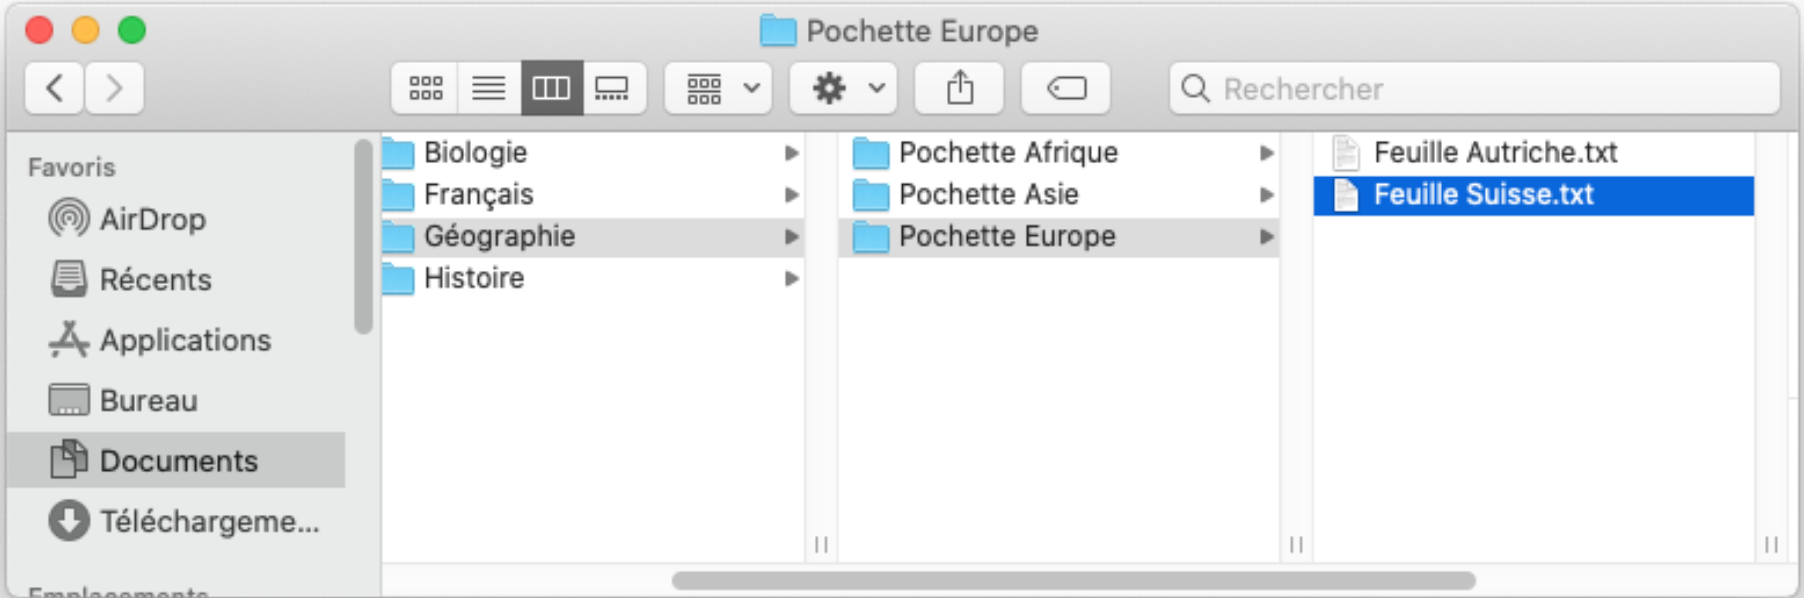
\includegraphics[width=15cm]{images/fichierMac}
\end{figure}

En mode console (textuel), la commande $ls$ permet de visualiser le contenu d'un répertoire et la commande $cd\ nom\_du\_dossier$ permet de se déplacer dans le dossier nommé nom\_du\_dossier.

\subsection{Microsoft Windows}

Sous Microsoft Windows, le chemin serait :

\begin{center}
{\bf C:$\backslash$Armoire de classeurs$\backslash$Géographie$\backslash$Pochette Europe
}
\end{center}

\begin{figure}[ht!]
\centering
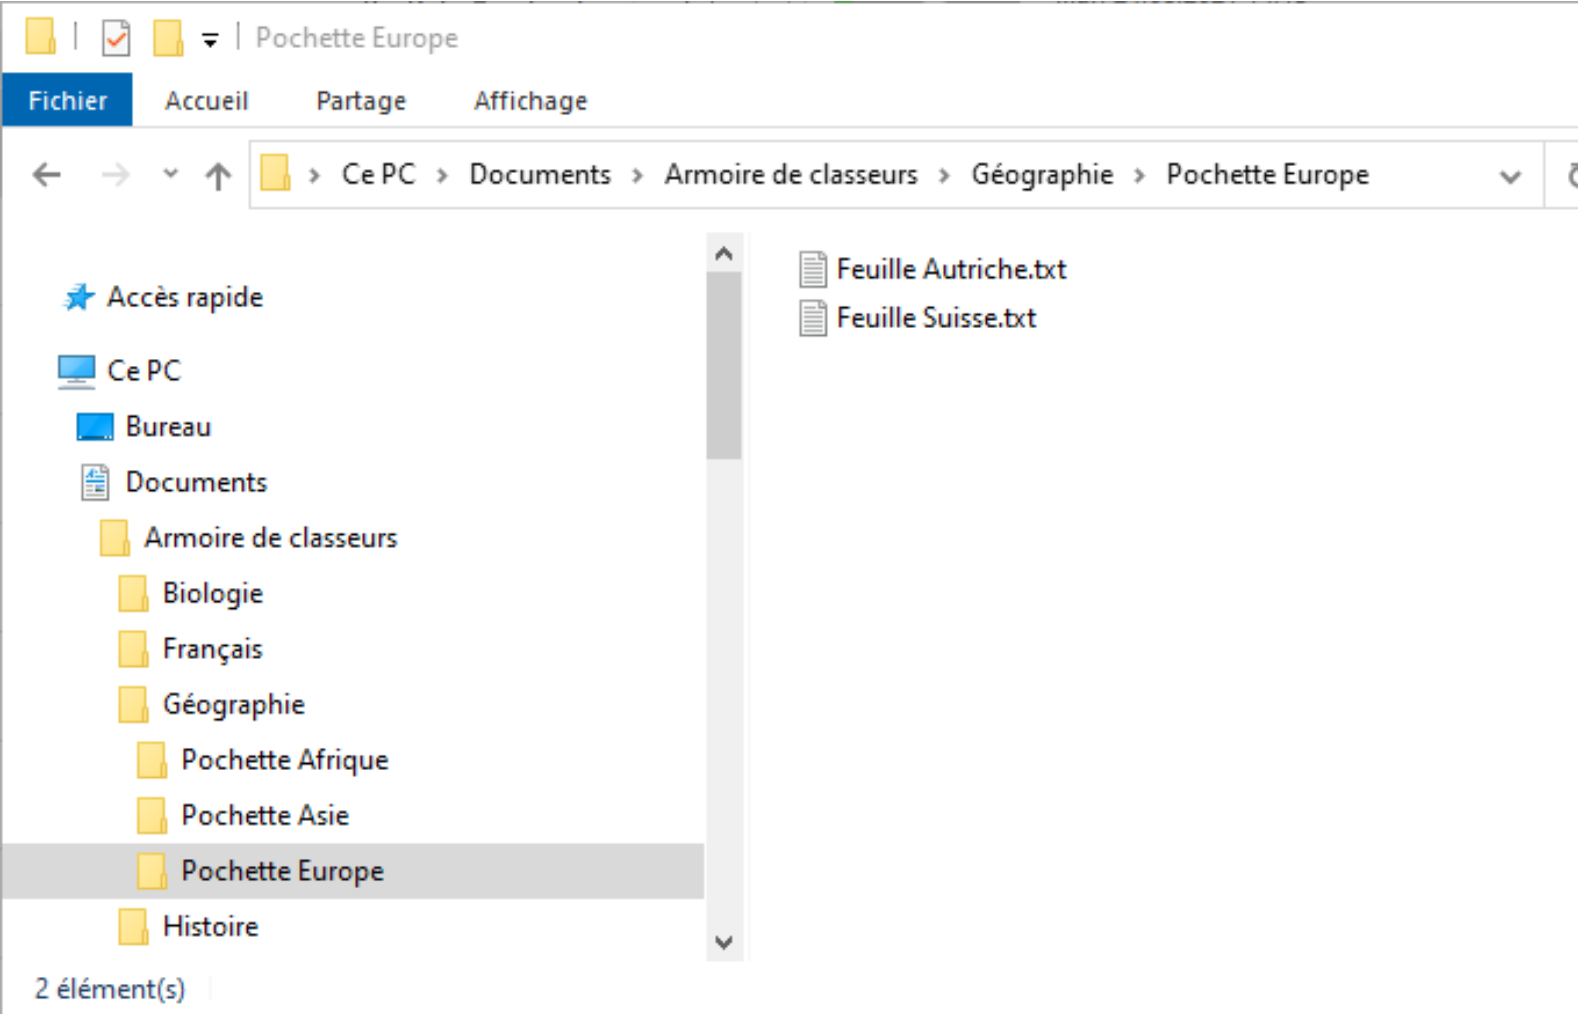
\includegraphics[width=11cm]{images/fichierWindows}
\end{figure}

Noter la différence entre les deux systèmes. Le caractère / qui délimite les niveaux pour GNU/Linux et macOS et le caractère $\backslash$ pour Microsoft Windows. Il y a aussi la lettre qui détermine la partition ou un périphérique (clé USB, lecteur DVD, etc.) alors que sous GNU/Linux et macOS, une partition est invisible à l’utilisateur·trice en étant considéré comme une branche de l’arbre. L'utilisation de lettre est une spécificité unique du système d'exploitation Microsoft Windows.

\section{Exercices}

\begin{exercice}
Se connecter sur www.eduge.ch puis aller sur le drive.
 Organiser le drive en sous fichier: Il devra y avoir un dossier principal nommé: Informatique et au moins 3 sous-dossiers appelés: Microbit, Python et Projet. 
 
 Le prochain petit programme fait en Microbit devra être sauvegardé sur le drive dans le dossier Microbit. 
\end{exercice}


\begin{exercice}
Dans moodle ou classroom, récupérez le fichier Exercice\_1\_fichier.zip et décompressez-le sur votre ordinateur.
Ouvrez le dossier "A\_Trier\_A\_Renommer", observez chaque fichier qu'il contient, renommez-les et déplacez-les dans le bon dossier. Renommez également les dossiers avec des noms corrects.
\begin{enumerate}
    \item Combien y a-t'il de dossiers dans le dossier Nourriture ?
    \item Combien y a-t'il de fichiers dans le dossier Legumes ?
    \item Quelle est la taille de l'image avec des carottes ?
    \item Quelle est l'extension de l'image avec des carottes ?
    \item Quelle est la taille du dossier Fruits ?
\end{enumerate}
\end{exercice}

\begin{exercice} *
Choisissez une photo prise avec votre smartphone. Donner quelques informations à son sujet en exploitant les métadonnées qui lui sont associées. Quand et où cette photo a-t-elle été prise? Sous quel nom et quel format est-elle stockée dans le smartphone? Quel est son poids? À quelles informations supplémentaires avons-nous accès?
\textit{Site pour lire les métadonnées : \url{https://www.verexif.com/fr/}}
\end{exercice}



\end{document}